\section{Case study: completely pivoted LU}

Linear algebra is ubiquitous in technical computing applications. At the same
time, the implementation of linear algebra libraries is generally considered a
difficult problem best left to the experts. A popular reference book for
numerical methods famously wrote, for example, that ``the solution of
eigensystems... is one of the few subjects covered in this book for which we do
\textit{not} recommend that you avoid canned routines''~\cite[Section 11.0, p.
461]{NumericalRecipesInC2e}. While much effort has been invested in making
numerical linear algebra libraries fast~\cite{LAPACK,FLAME,BLIS}, one
nevertheless will occasionally need an algorithm that is not implemented in a
standard linear algebra librasy.

One such nonstandard algorithm is the completely pivoted LU factorization. This
algorithm is not implemented in standard linear alagebra libraries in
LAPACK~\cite{LAPACK}, as the conventional wisdom is the gains in numerical
stability in complete pivoting is no generally worth the extra effort over
other variants such as partial pivoting~\cite{Golub2013}.  Nevertheless, users
may want complete pivoting for comparison with other algorithms for a
particular use case. For example, one may be interested in comparing the
results of an infinite dimensional LU factorization to its finite-dimensional
approximation, in which case only the completely pivoted LU is defined in both
cases~\cite{Townsend2015}.

In this section, we consider various implementation of completely pivoted LU in
pure Julia. First, we implement the algorithm na\"ively as a direct translation
from the textbook description, and compare the performance with na\"ive
implementations in other high level languages that are commonly used for
technical computing, such as MATLAB, Octave, Python/NumPy, and R. Second, we
rewrite the na\"ive Julia implementation for better performance, and
demonstrate the effects of each transformation on execution time. We believe
that this work flow reflects typical use cases of high level dynamic languages,
where users first write na\"ive but verifiably correct implementations, then
rewrite the implementation until sufficient performance can be achieved.



\subsection{Na\"ive textbook implementation}

Algorithm~\ref{alg:lucompletepiv} presents the textbook description of the LU
factorization with complete pivoting~\cite[Algorithm 3.4.3 (Outer Product LU
with Complete Pivoting), p. 132]{Golub2013}, and below it a direct translation
into a na\"ive Julia implementation. This algorithm is presented in MATLAB-like
pseudocode, and contains a mixture of scalar \lstinline|for| loops and
MATLAB-style vectorized indexing operations that describe various subarrays of
the input matrix $A$. Additionally, there is a description for the subproblem
of finding the next pivot at the start of the loop. Furthermore, the pseudocode
uses the $\leftrightarrow$ operation, denoting swaps of various rows and
columns of $A$. To translate these pieces into Julia, we used the builtin
\lstinline|indmax| function to

\begin{algorithm}

\caption{Top: Textbook pseudocode describing the $LU$ factorization with
complete pivoting~\cite[Algorithm 3.4.3 (Outer Product LU with Complete
Pivoting), p. 132]{Golub2013}. The matrix $A$ is overwritten in-place with the
$LU$ factors, with $rowpiv$ and $colpiv$ containing the row and column pivots
respectively.
Bottom: An implementation of $LU$ factorization with complete pivoting in Julia,
which returns the result as a tuple. The ! at the end of the function name is
convention for a function with side effects (in this case, mutating $A$). The
implementation defines a custom function $\leftrightarrow$ which is allowed to
be used as an operator in infix position. Other Unicode characters such as
Greek letters and the $\ne$ operator are allowed in Julia code, allowing for
close notational correspondence with the textbook description of the algorithm.}
\label{alg:lucompletepiv}

\begin{algorithmic}
\For {$k = 1:n - 1$}

    Determine $\mu, \lambda$ where $k \le \mu \le n$,  $k \le \lambda \le n$, so

    $\quad\left|A(\mu, \lambda)\right| = \max\{ \left|A(i, j)\right| : i=k:n, j=k:n \}$

    $rowpiv(k) = \mu$

    $A(k, 1:n) \leftrightarrow A(\mu, 1:n)$

    $colpiv(k) = \lambda$

    $A(1:n, k) \leftrightarrow A(1:n, \lambda)$

    \If{$A(k,k) \ne 0$}

        $\rho = k+1:n$

        $A(\rho, k) = A(\rho, k)/A(k, k)$

        $A(\rho, \rho) = A(\rho, \rho) - A(\rho, k) A(k, \rho)$
    \EndIf
\EndFor
\end{algorithmic}

\hrulefill

\begin{lstlisting}
function lucompletepiv!(A)
	n=size(A, 1)
	rowpiv=zeros(Int, n-1)
	colpiv=zeros(Int, n-1)
	for k=1:n-1
		Asub = abs(A[k:n, k:n]) #Search for next pivot
		$\mu$, $\lambda$ = ind2sub(size(Asub), indmax(Asub))
		$\mu$ += k-1; $\lambda$ += k-1
		rowpiv[k] = $\mu$
		A[[k, $\mu$], 1:n] = A[[$\mu$, k], 1:n]
		colpiv[k] = $\lambda$
		A[1:n, [k, $\lambda$]] = A[1:n, [$\lambda$, k]]
		if A[k,k] $\ne$ 0
			$\rho$ = k+1:n
			A[$\rho$, k] = A[$\rho$, k]/A[k, k]
			A[$\rho$, $\rho$] = A[$\rho$, $\rho$] - A[$\rho$, k] * A[k, $\rho$]
		end
	end
	return (A, rowpiv, colpiv)
end
\end{lstlisting}

\end{algorithm}


\begin{figure*}
	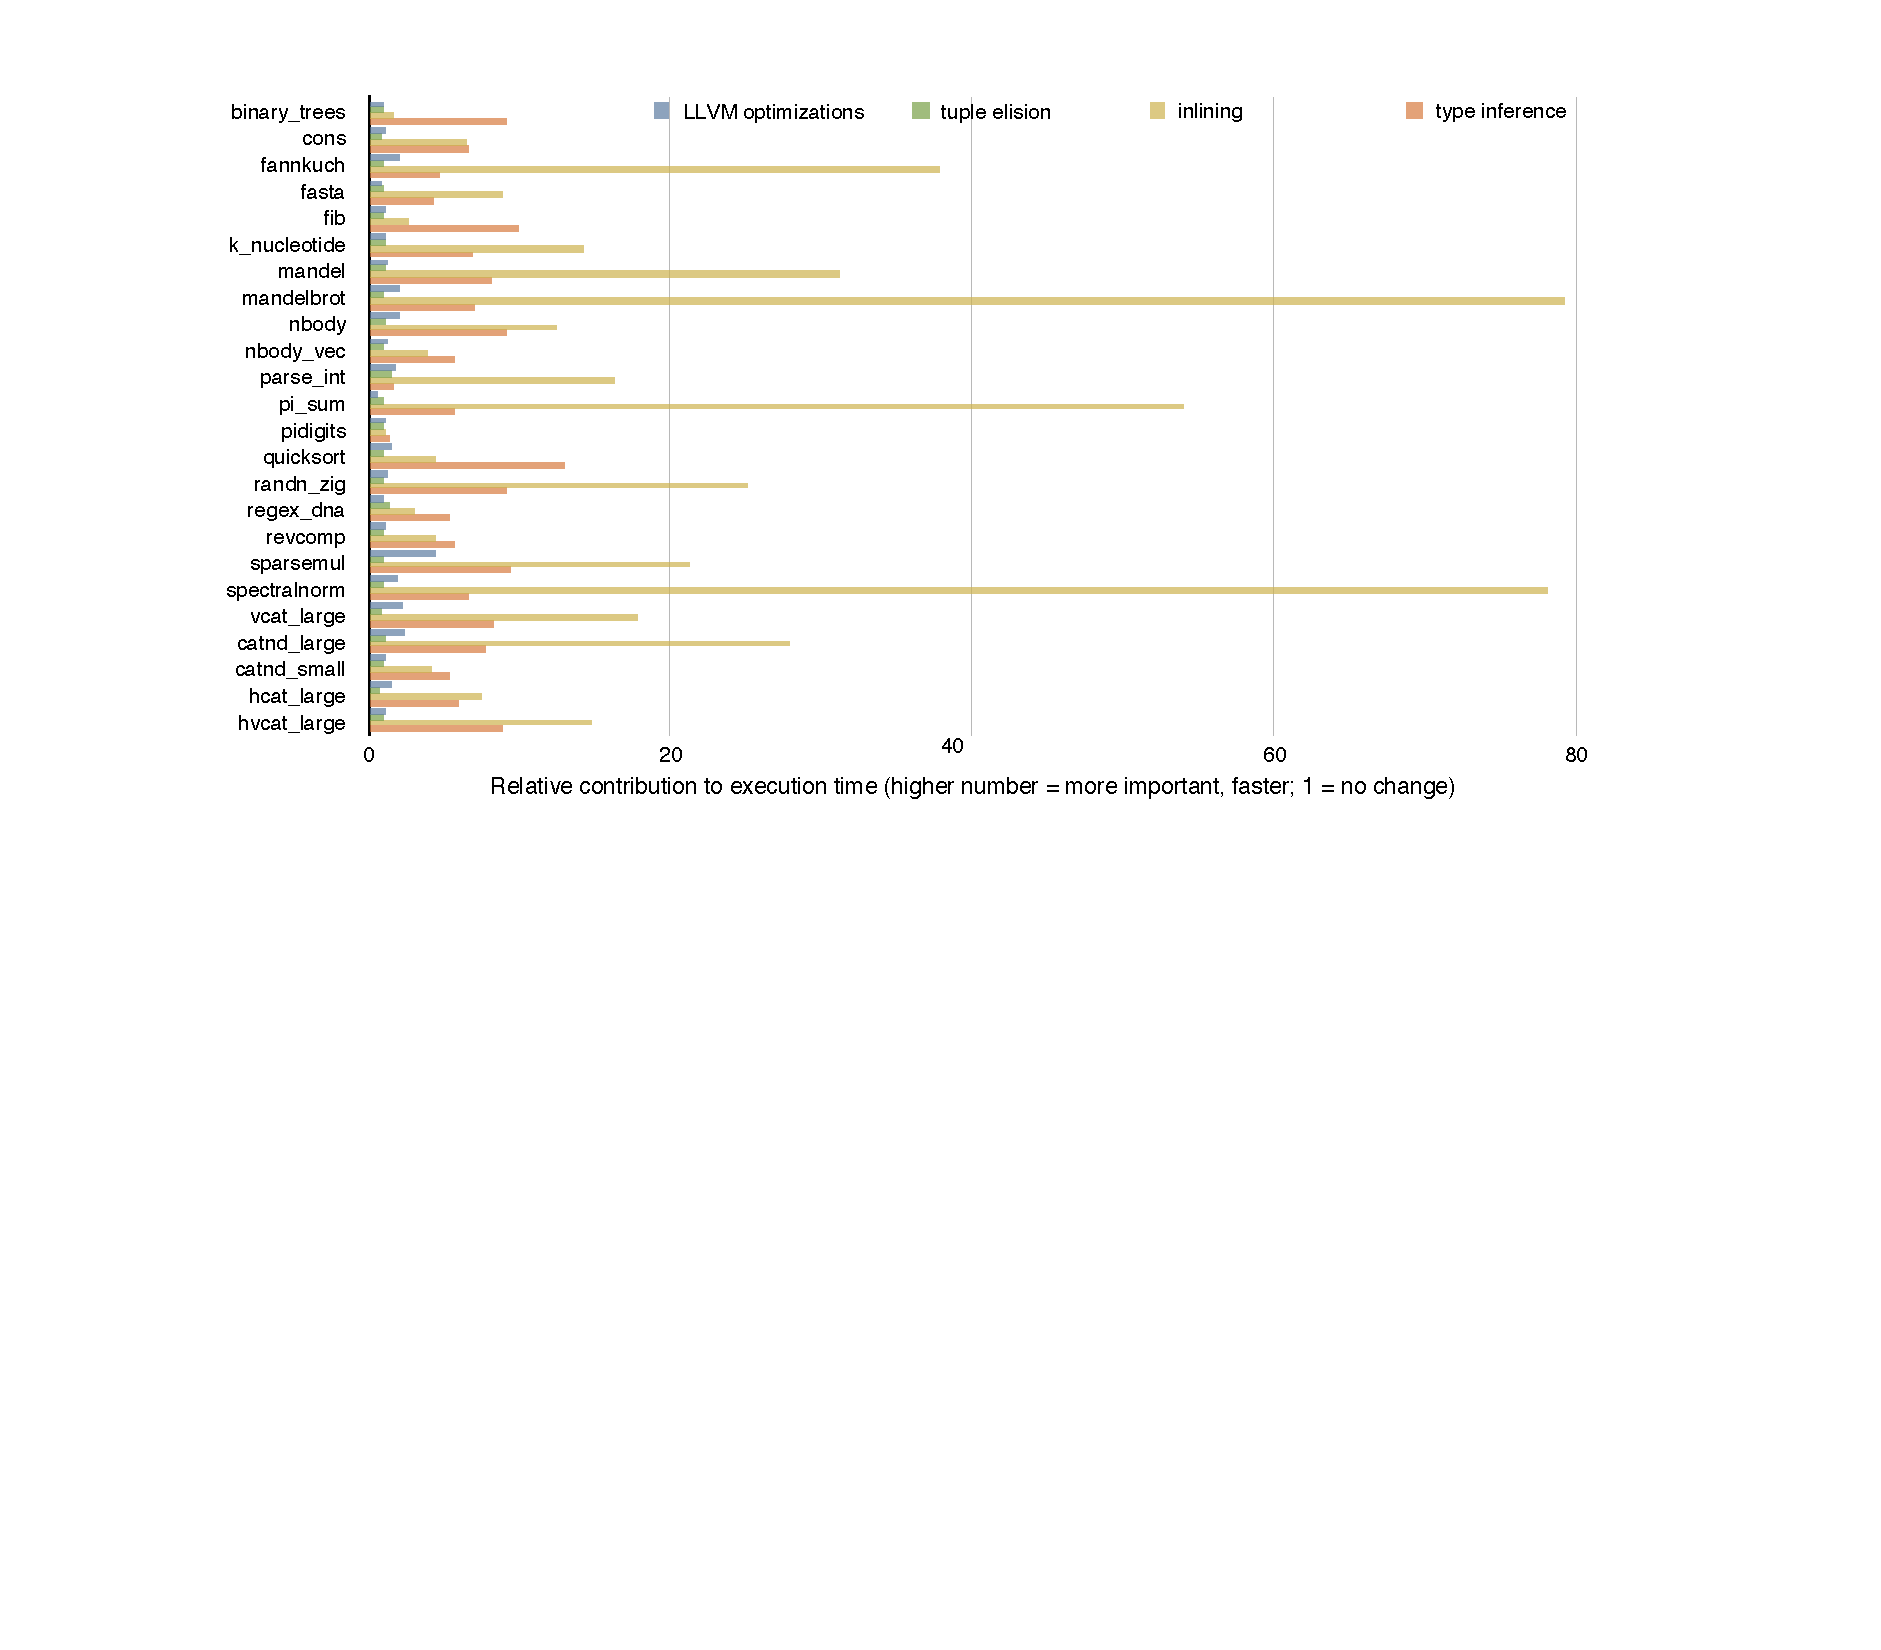
\includegraphics[width=\textwidth]{fig-timings}
	\caption{Relative contributions of various optimization passes to
	performance of Julia code implementing a representative collection
	of benchmarks. Bars from top to bottom represent: LLVM
	optimizations, tuple elision, function inlining, and type inference.}
	\label{fig:timings}
\end{figure*}



\subsection{Improving the performance of a na\"ive implementation}


